
%title page
\begin{frame}
\titlepage
\end{frame}

\section{High-energy \texorpdfstring{$\gamma$}{gamma} sources}

\begin{frame}{Why to study?}
  \begin{itemize}
    \item $\gamma$:
    \begin{itemize}
	\item are not deflected by interstellar magnetic fields $\Rightarrow$ can be tracked to their origin;
	\item can be used for point sources search;
	\item are able to provide answers about the Galactic cosmic ray propagation;
	\item $\gamma$-ray flux study could bring us insights on cosmic rays acceleration mechanisms.
    \end{itemize}
    \item high-energy $\gamma$ (above 100~TeV):
    \begin{itemize}
	\item not so well-investigated because of flux intensity decrease for all CR particles at higher energies;
	\item are supposed to be produced by black holes, neutron stars, supernova remnants, super-bubbles / star-forming regions / young massive star clusters;
	\item could improve our understanding about properties of matter in extreme states that cannot be studied in laboratories.
    \end{itemize}
  \end{itemize}
\end{frame}

\begin{frame}{HAWC high-energetic $\gamma$-ray sources}

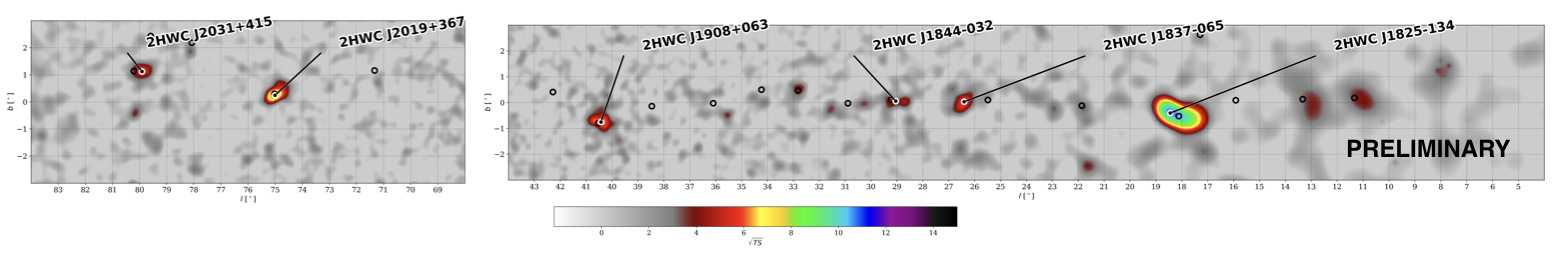
\includegraphics[width=1\textwidth]{pics/Malone0.png}
\begin{itemize}
  \item six sources in the Galactic plane that emit above 56~TeV.
\end{itemize}
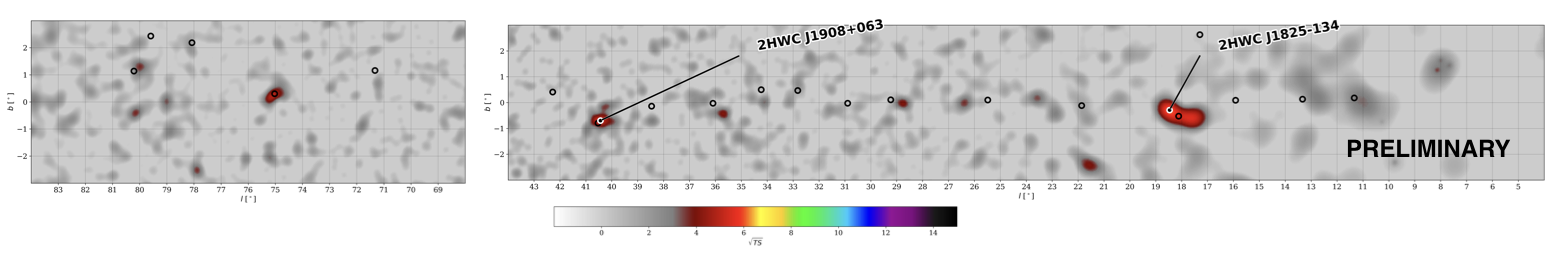
\includegraphics[width=1\textwidth]{pics/Malone1.png}
\begin{itemize}
  \item two of them continue to emit past 100~TeV.
\end{itemize}

\end{frame}

\begin{frame}{CARPET results-1}

\end{frame}

\begin{frame}{CARPET results-2}

\end{frame}
